
\section{Methods}\label{sec:methods}


\subsection{Dataset}

The project focuses on uncovering the depression status of individuals using EATD-Corpus \cite{shen2022automatic}, which contains audio and extracted transcripts of responses from depressed and non-depressed volunteers. For this study, we will only utilize the audio recordings for our analysis.

Each volunteer responded to three randomly selected interview questions and completed an SDS (Self-Rating Depression Scale) questionnaire which assesses common characteristics of depression. The raw SDS score obtained from this questionnaire is an indicator of depression severity. In Chinese individuals, the SDS score multiplied by 1.25 (i.e., raw SDS score × 1.25) suggests depression if it is greater than or equal to 53. Consequently, to form our classification problem we map the target classes to 0 (non-depressed) if their score is less than 53, and to 1 (depressed) otherwise.

The EATD-Corpus dataset comprises audio recordings derived from interviews conducted with 162 student volunteers who received counseling, particularly within the Chinese context to support research in depression detection. The training set contains data from 83 volunteers (19 depressed and 64 non-depressed), whereas the validation set contains data from 79 volunteers (11 depressed and 68 non-depressed). The total duration of response audios in the dataset amounts to approximately 2.26 hours, having a sample rate of 16KHz.

In the original EATD-Corpus paper, however, they do not respect the same data orientation through their learning process. Instead, the performance of their proposed method is further evaluated with 3-fold cross-validation. The training and validation samples in the dataset are all merged into a single dataset, and then divided into three groups where two of which are used for training and the other one for testing. This results in 108 training and 54 validation samples. The results reported are an average performance across the folds.


\subsection{Preprocessing}

Before delving into the classification algorithms, it is important to preprocess and cleanse the data to ensure optimal performance and reliability throughout the analysis. 

EATD-Corpus also provides the preprocessed version of the audio files, where they mute audios shorter than one second, trim the silent sections at the beginning and end of each recording, and eliminate the background noise using RNNoise \cite{valin2018hybrid} with default parameters. We will attempt to use the same preprocessed files to ensure compatibility when comparing the algorithms.

For each sample, there are three different responses recorded in files named \texttt{positive\_out.wav}, \texttt{neutral\_out.wav}, and \texttt{negative\_out.wav}. These recordings have different duration and vary from 2 seconds to a minute long.

To address this variability, in the original EATD-Corpus paper, the authors extracted the Mel spectrogram features from each of these responses, adopted NetVLAD \cite{arandjelovic2016netvlad} to generate
audio embeddings of the same length from Mel spectrograms, and concatenated all these embeddings together.

In our approach, however, we separated our preprocessing step from the feature extraction phase. We first extracted and concatenated the waveforms from \texttt{positive\_out.wav}, \texttt{neutral\_out.wav}, and \texttt{negative\_out.wav}. These concatenated waveforms were then directly used in the statistical feature extraction. However, to ensure uniform waveform lengths for other proposed feature extraction techniques, we applied zero-padding to the right side based on the maximum duration observed. This process is illustrated in Fig.~\ref{fig:zeropad}.

\begin{figure}[!t]
    \centerline{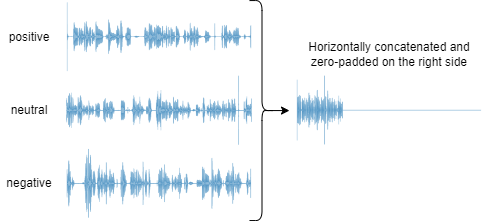
\includegraphics[width=\columnwidth]{images/zeropad.png}}
    \caption{Waveform Concatenation and Zero-Padding}
    \label{fig:zeropad}
\end{figure}


\subsection{Feature Extraction}

Assuming a frame size of 512 and overlapping frames with a hop size of 256, we attempt to perform three different experiments with different feature selection methods: Log-Mel spectrogram features, Mel-frequency cepstral coefficients (MFCC), and custom statistical features.

\subsubsection{Log-Mel Spectrogram Features}

Using the zero-padded waveforms and the windowing characteristics mentioned earlier, Mel-spectrogram features with 80 mel frequency bands were extracted by the \texttt{librosa} \cite{mcfee2015librosa} library from the audio waveform data for time-frequency analysis. The resulting mel-spectrogram was then converted to a logarithmic scale to enhance its representation for further analysis. The dimensions of the final feature space resulted in samples of size \texttt{(1, 80, 18551)}, having mono audio channels. A sample extracted log-mel spectrogram can be seen in Fig.~\ref{fig:logmel}

\begin{figure}[!t]
    \centerline{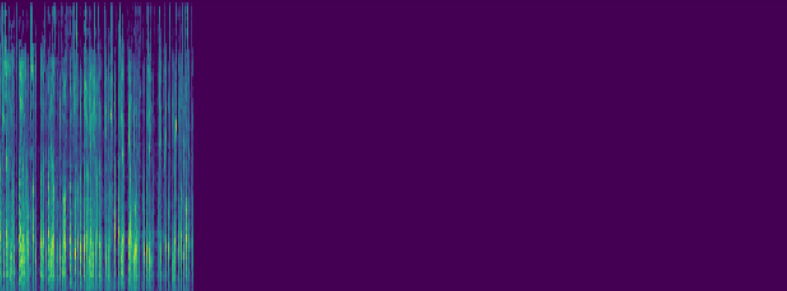
\includegraphics[width=\columnwidth]{images/logmel.png}}
    \caption{Log-Mel Spectrogram Features Extracted from Waveforms}
    \label{fig:logmel}
\end{figure}

\subsubsection{MFCC Features}

Similar to the extraction of Log-Mel spectrogram features, the MFCC extraction involved calculating 13 coefficients over the specified frame and hop lengths (512 and 256, respectively). To capture dynamic changes in the MFCCs over time, first-order and second-order temporal derivatives were also computed and concatenated vertically on top of the MFCC features to form a comprehensive feature set for subsequent analysis. The resulting dimensions of the MFCCs formed samples of size \texttt{(1, 39, 18551)}. A sample extracted MFCC can be seen in Fig.~\ref{fig:mfcc}

\begin{figure}[!t]
    \centerline{
\includegraphics[width=\columnwidth]{images/mfcc.png}}
    \caption{MFCC Features Extracted from Waveforms}
    \label{fig:mfcc}
\end{figure}

\subsubsection{Statistical Features}

We experimented with another set of simplified features in our settings which was robust to variation in audio lengths, not requiring the zero-padding. As discussed in \cite{low2020automated}, different acoustic features can be effective in identifying psychiatric disorders such as depression. For each frame of the given sample, using the same framing characteristics as previously described, we computed several variables: Energy (1 value per frame), Zero-Crossing Rate (1 value per frame), and the first 13 Mel-frequency cepstral coefficients (MFCCs) along with their corresponding first-order and second-order derivatives (39 values per frame in total). This process yielded a comprehensive list of features for each frame, which we subsequently subjected to statistical analyses including average, variance, minimum, and maximum calculations across all frames for each feature. This process results in acquiring samples of size \texttt{(164)}.

In order to reproduce the results of the EATD-Corpus, we will also attempt to store their log-mel features. Acoustic features extracted by the authors of EATD-Corpus have the dimensions of \texttt{(3, 256)} across all the samples.


\subsection{Data Augmentation and Resampling}

Depression datasets often suffer from significant data imbalance, where the number of samples in the non-depressed class dominates over the depressed class. This imbalance can lead to a bias towards the majority class during model training. To overcome this issue, the authors of EATD-Corpus used an augmentation and resampling technique to rearrange the order of the volunteers' three responses, and then resample these rearranged samples to increase the size of the depressed class and create new training samples. Since there are 6 ways of response rearrangement for each individual, the size of the depressed class can be enlarged by a factor of 6.

However, in our experiment, we do not follow their methodology to overcome the data imbalance. We believe that this approach naively introduces fake and augmented samples in the dataset, preventing us from reporting realistic evaluation measurements on the dataset.


\subsection{Classification Methods}

Three different experiments were investigated to be compared with the reproduced results from the EATD-Corpus. In order to achieve this, we first utilized the exact code reported by the EATD-Corpus GitHub repository \cite{shen2022icassp} and used the same experiment setup to replicate their results. Then, we implemented our own set of classifiers with specialized feature extraction techniques, which are summarized below:

\input{figs/table:cnn}

\begin{figure}[!t]
    \centerline{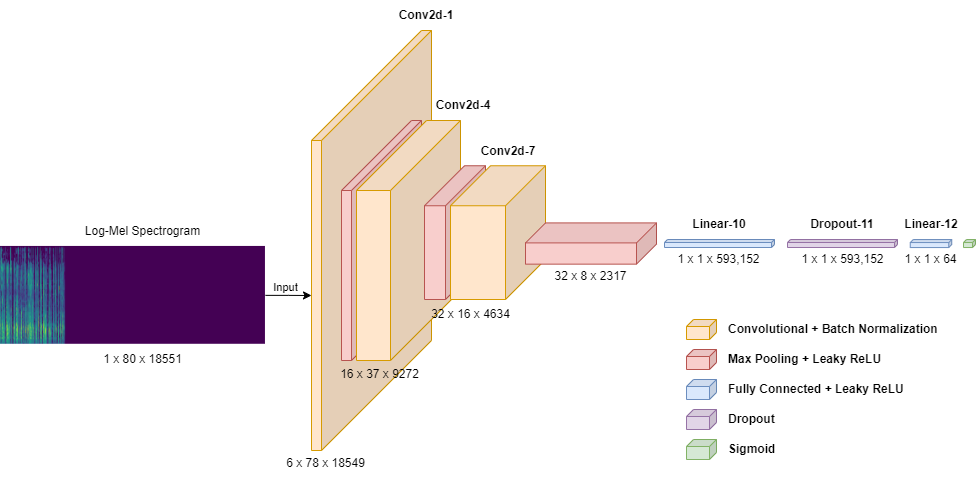
\includegraphics[width=\columnwidth]{images/CNN.png}}
    \caption{Proposed CNN Architecture for Log-Mel Features}
    \label{fig:cnn}
\end{figure}

\input{figs/table:cnn_lstm}

\begin{figure}[!t]
    \centerline{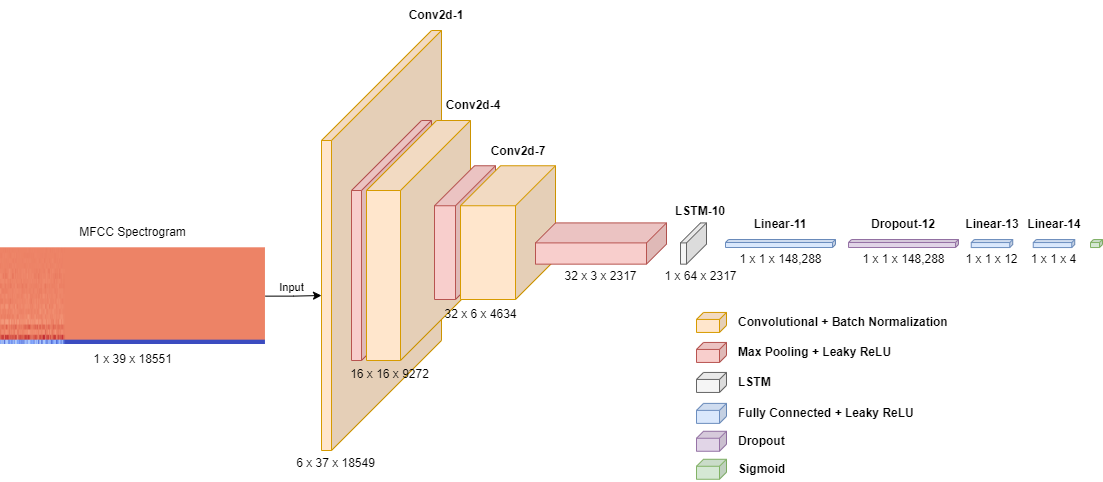
\includegraphics[width=\columnwidth]{images/CNN-LSTM.png}}
    \caption{Proposed CNN-LSTM Architecture for MFCC Features}
    \label{fig:cnn_lstm}
\end{figure}

\subsubsection{CNN Architecture for Log-Mel Features}

We will input the log-mel features extracted from the audio files into a CNN network specifically designed for depression detection. Throughout the network, convolution layers with 6, 16, and 32 channels are used respectively, all with a kernel size of \texttt{(3x3)}. In order to perform downsampling and dimensionality reduction, max-pooling layers with kernel size of \texttt{(2x2)} and stride of 2 are employed. To speed up the training process and improve the generalization capability, batch normalization is adopted. Leaky ReLU is utilized as the activation function of these convolutional layers. Then, the resulting feature maps are flattened and fed into a fully connected (FC) layer (with Leaky ReLU activation) with only one hidden layer of 64 neurons, through which a Dropout layer is used to enhance the regularization and prevent overfitting. Finally, at the last layer, a single neuron goes through a Sigmoid activation function reflecting the likelihood of the individual experiencing depression.

In order to minimize the error and fit the training set, the Binary Cross Entropy loss function in conjunction with the Adam optimizer. The learning rate was set to \texttt{1e-6}, and the model was trained across 40 epochs using a batch size of 8.

Table \ref{table:cnn} represents the proposed CNN architecture having inputs of size \texttt{(1, 80, 18551)}. Fig.~\ref{fig:cnn} visualizes the network architecture for better intuition.

\subsubsection{CNN-LSTM Architecture for MFCC Features}

LSTM models have been shown to be effective in the domain of depression detection \cite{al2018detecting}. Using another architecture, we will attempt to train a CNN-LSTM network on the extracted MFCC features to classify the individuals into depressed and non-depressed classes. The convolutional layers preserve the same characteristics as the previous network, having the same dimensionality, pooling layer, batch normalization, and activation function. Then, an LSTM layer with 64 hidden dimensions accepts the sequences flowing from the previous layer. The outputs of the LSTM layer are then flattened and fed to a fully connected (FC) network with two hidden layers, having 12 and 4 hidden neurons respectively. The Dropout layer is also utilized, and the last single neuron represents the depression probability similar to the previous network through a Sigmoid activation function.

Similar to the previous network, we utilized the Binary Cross Entropy loss function along with the Adam optimizer to minimize error and fit the training set. The learning rate was set to \texttt{5e-6}, and training was conducted over 50 epochs with a batch size of 8.

Table \ref{table:cnn_lstm} represents the CNN-LSTM architecture having inputs of size \texttt{(1, 39, 18551)}. Fig.~\ref{fig:cnn_lstm} demonstrates this architecture in more detail.

\subsubsection{Traditional Classifiers}

Inspired by the effective classical models used in the domain reported in \cite{wu2023automatic}, we use the custom statistical features extracted from the audio files and adopt different traditional classifiers to be able to evaluate the effectiveness of our approach.

\begin{itemize}[\IEEEsetlabelwidth{Z}]
    \item K-Nearest Neighbors (KNN) classifier is used with the following hyper-parameter settings: \texttt{\{algorithm:"auto", leaf\_size:10, n\_neighbors:5, p:1, weights:"uniform"\}}

    \item Decision Tree classifier is used with the following hyper-parameter settings: \texttt{\{criterion:"gini", max\_depth:15, max\_features:"log2", min\_samples\_leaf:1, min\_samples\_split:2\}}

    \item Random Forest classifier is used with the following hyper-parameter settings: \texttt{\{criterion:"gini", max\_depth:5, min\_samples\_leaf:1, n\_estimators:20\}}

    \item AdaBoost classifier is used with the following hyper-parameter settings: \texttt{\{algorithm:"SAMME.R", learning\_rate:1.0, n\_estimators:50\}}

    \item Multi-Layer Perceptron (MLP) classifier is used with the following hyper-parameter settings: \texttt{\{activation:"relu", alpha:0.0001, hidden\_layer\_sizes:[60], learning\_rate:"adaptive", max\_iter:1000, solver:"adam"\}}
\end{itemize}


\subsection{Evaluation Metrics}

In order to provide a comparison between the different classification methods discussed, we will use the following metrics:

\begin{itemize}[\IEEEsetlabelwidth{Z}]
    \item Accuracy: The accuracy metric measures the proportion of correctly classified instances (both depressed and non-depressed) among the total number of instances in the dataset. It is calculated as:

    \begin{equation}
        \text{Accuracy} = \frac{TP + TN}{TP + TN + FP + FN}
    \end{equation}

    \item Precision: Precision measures the proportion of correctly predicted depressed instances among all predicted depressed instances. It is calculated as:

    \begin{equation}
        \text{Precision} = \frac{TP}{TP + FP}
    \end{equation}

    \item Recall: Recall (Sensitivity or True Positive Rate) measures the proportion of correctly predicted depressed instances among all actual depressed instances. It is defined as:

    \begin{equation}
        \text{Recall} = \frac{TP}{TP + FN}
    \end{equation}

    \item F1-Measure: The F1 measure (F1 score) is the harmonic mean of precision and recall, providing a balanced evaluation of the model's performance. It is computed as:

    \begin{equation}
        \text{F1} = 2 \times \frac{\text{Precision} \times \text{Recall}}{\text{Precision} + \text{Recall}}
    \end{equation}

    where TP (True Positive) is the number of correctly predicted depressed instances, TN (True Negative) represents the number of correctly predicted non-depressed instances, FP (False Positive) denotes the number of non-depressed instances incorrectly predicted as depressed, and FN (False Negative) demonstrates the number of depressed instances incorrectly predicted as non-depressed.

\end{itemize}